\documentclass[twoside,a4paper,openright,titlepage,draft]{ctexrep}
\usepackage[final]{graphicx}
\usepackage{subfig}
% \usepackage{subcaption}
\usepackage{extarrows}
\usepackage{multicol}
\usepackage{float}
\usepackage{amsmath}
\usepackage{subfig}
\usepackage{cancel}
\usepackage{wrapfig}
\graphicspath{{./pictures}}
\setcounter{secnumdepth}{3}

\begin{document}
\section{共漏极放大电路}

\subsection{前言}
\par
对于一个共源极放大电路来说,输出阻抗很大,但是当负载阻抗很小的时候,就无法驱动负载了。
所以要引入源极跟随器(Source Follower),也就是共漏极放大器。\\

\begin{figure}[H]
    \centering
    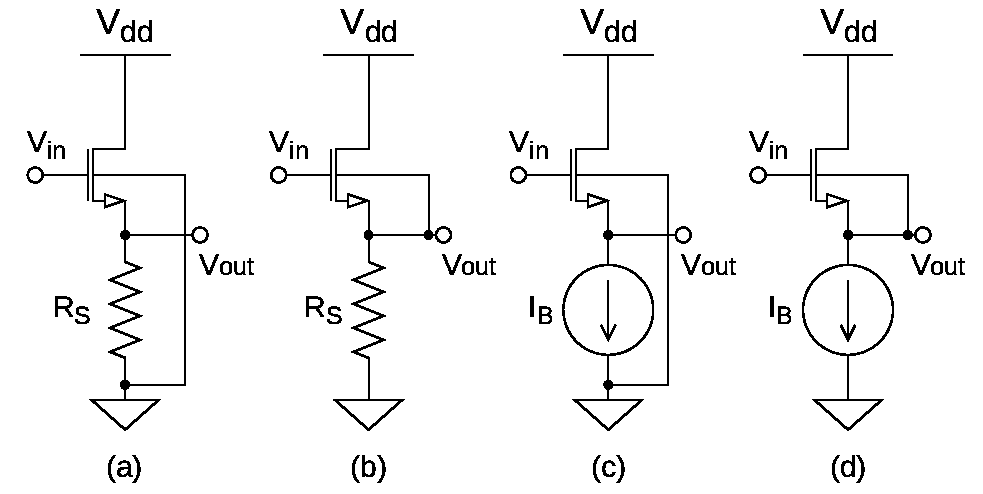
\includegraphics[width=\textwidth]{sourcefollower.eps}
    \caption{源极跟随器}
    \label{fig:源极跟随器}
\end{figure}

\subsection{电阻负载的源极跟随器}
\subsubsection{增益Gain}
\begin{multicols}{2}
    \begin{figure}[H]
        \centering
        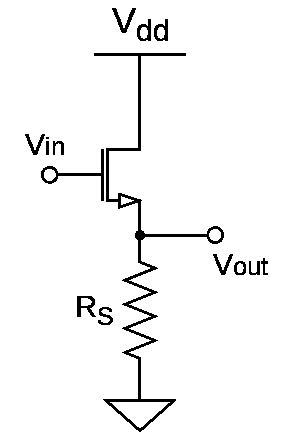
\includegraphics[height=40mm]{sourcefollower2.eps}
        \caption{电阻负载的源极跟随器}
        \label{fig:电阻负载的源极跟随器}
    \end{figure}
    \columnbreak
    \paragraph{大信号法:}
    \begin{align}
        V_{out} &= \frac{1}{2}\mu_n C_{ox}\frac{W}{L}(V_{in} - V_{TH} - V_{out})^2R_S \notag \\
        \frac{\partial V_{out}}{\partial V_{in}} &= \frac{1}{2}\mu_nC_{ox}\frac{W}{L}2(V_{in} - V_{TH} - V_{out})\notag \\
        &(1-\frac{\partial V_{TH}}{\partial V_{in}}-\frac{\partial V_{out}}{\partial V_{in}})R_S \notag
    \end{align}
    太复杂了,用小信号法
\end{multicols}
\paragraph{小信号法:}
如图\ref{fig:小信号模型}:
\begin{figure}[H]
    \centering
    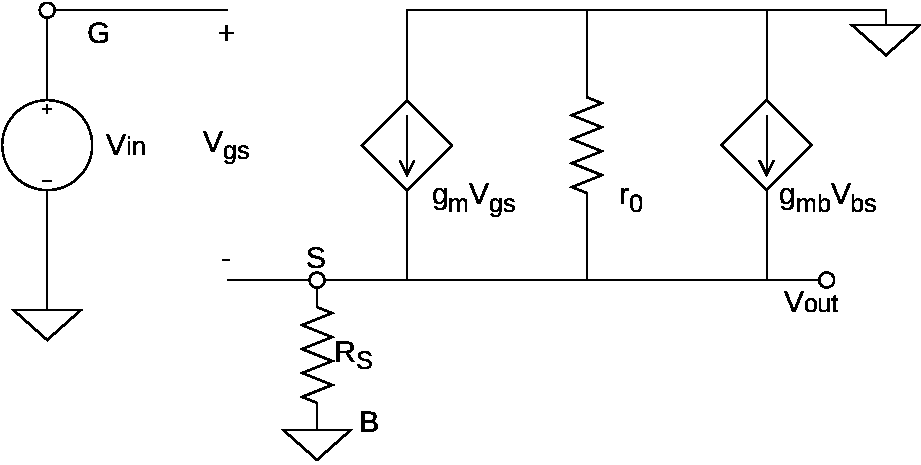
\includegraphics[width=0.8\columnwidth]{smallsignal.eps}
    \caption{小信号模型}
    \label{fig:小信号模型}
\end{figure}
\begin{align}
    &\begin{cases}
        \frac{V_{out}}{R_S} &= g_mV_{gs} + \frac{V_{ds}}{r_0} + g_mV_{bs} \\
        V_{gs} &= V_{in} - V_{out} \\
        V_{ds} &= - V_{out} \\
        V_{bs} &= -V_{out} \\
    \end{cases} \\
    \vspace{2mm}
    &A_v = \frac{V_{out}}{V_{in}} = \frac{g_m}{g_m + g_{mb} + \frac{1}{r_0} + \frac{1}{R_S}}
\end{align}
增益小于1(Gain $<1$)。
当忽略$\lambda$,$\gamma$的时候,增益Gain为1。
\subsubsection{小信号输出电阻:}
\begin{equation}
    R_{out} = R_S\ ||\ (r_0\ ||\ \frac{1}{g_m + g_{mb}})
\end{equation}
\subsubsection{Application:}
\paragraph{1、Level Shifter电平转换器}
如图\ref{fig:电平转换器}:
\begin{figure}[H]
    \centering
    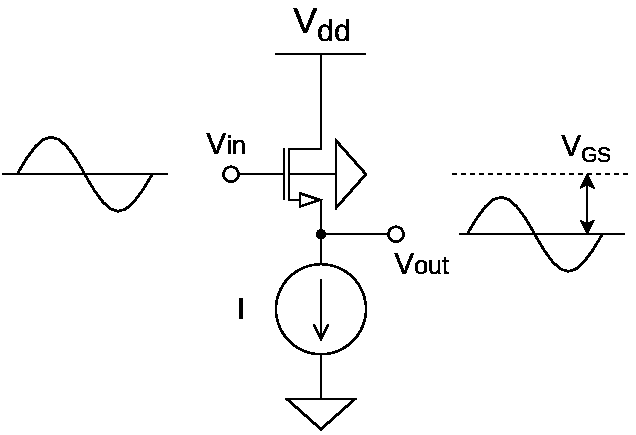
\includegraphics[height=40mm]{levelshifter.eps}
    \caption{电平转换器}
    \label{fig:电平转换器}
\end{figure}
\paragraph{2、Buffer}
用于最后一级驱动小电阻负载。

\end{document}